\noindent
{\bf Abstract:}
The problem of labeling the edges present in a single color image as convex, concave, and occluding 
entities is one of the fundamental problems in computer vision~\cite{mild-sugihara}. It has been shown 
that this information can contribute to segmentation, reconstruction and recognition problems. Recently, 
it has been shown that this classification is not straightforward even using RGBD data. This makes us 
wonder whether this apparent simple cue has more information than a depth map? In this paper, 
we propose a novel algorithm using random forest for classifying edges into convex, concave and 
occluding entities. We release a data set with more than 500 RGBD images with pixel-wise ground 
labels. Our method produces promising results and achieves an F-score of $0.84$ on the data set.
[We first solve the problem using scanned 3D models. Then we move on to use stereo images which is more difficult.]

\noindent
{\bf Introduction:}
Edges in an image often correspond to depth discontinuities at object boundaries (occlusion 
edges) or normal discontinuities (convex or concave edges). In addition, there could be 
planar edges that are within planar regions. Figure~\ref{fig:EdgeLabeling} shows an image 
containing different types of edges. Note that planar edges may result from shadows, reflection, 
specularities and albedo variations. In classical line labeling with synthetic line 
drawings, we do not have any planar edges as the purpose of edge labeling has always been to 
classify the depth edges as occluding, convex and concave. However, in real images planar 
edges occur more frequently than others. This paper studies the problem of classifying boundaries 
from RGBD data. In many 3D models obtained using RGBD sensors or multi-view reconstruction techniques, 
we typically have very noisy 3D point cloud near the boundaries. This is because most stereo 
reconstruction algorithms and structured light techniques are known to provide noisy reconstruction 
near the boundaries. This makes the labeling problem challenging. 

\begin{figure}[t]
\centering
       \subfigure[RGB Image]{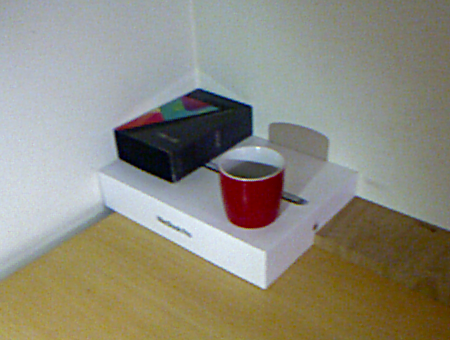
\includegraphics[width=0.32\columnwidth]{images/Im1-RGB.png}} \hfill
       \subfigure[Edge Types]{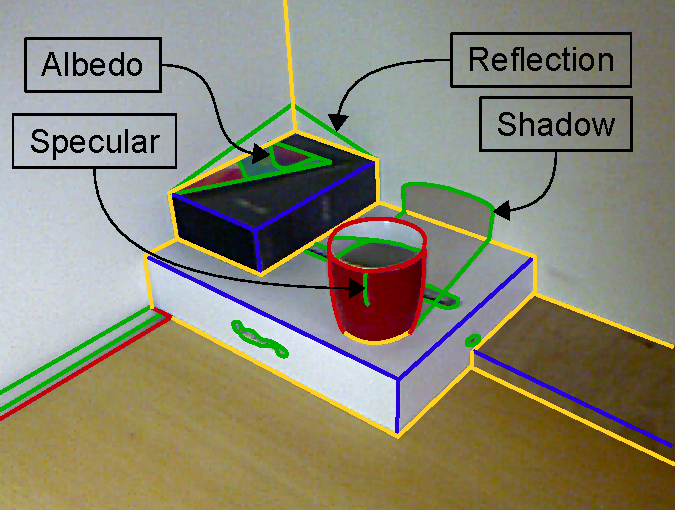
\includegraphics[width=0.32\columnwidth]{images/Im1-Labelled-1.pdf}} \hfill
       \subfigure[Depth Map]{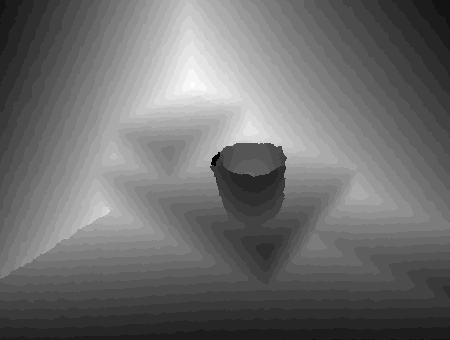
\includegraphics[width=0.32\columnwidth]{images/Im1-Depth.png}} \\
\caption{\it The edges in (a) are marked in (b) with the color code: red (occluding), green (planar),
blue (convex), and yellow (concave). Planar edges are caused by different phenomena as marked.
(c) shows the Kinect depth map (note the depth quantization artifacts).}
\label{fig:EdgeLabeling}
\end{figure}

\noindent


\section{Method}
\section{Contour Labeling}

We use both image and depth cues to infer the labels of edge pixels. We start with a set 
of edge pixels obtained from an edge detection algorithm and the goal is to assign one 
of the four labels to each of these edge pixels. However, to improve computational efficiency 
and to overcome noise in the data, we link similar connected edge pixels in a neighborhood 
into contour segments. The process is carried out using an edge linking algorithm that 
combines connected edge pixels into a link as long as the curvature of the link is within 
a threshold. Each edge pixel is uniquely mapped to one of the contour segments. Each contour 
segment $c_i$ corresponds to a set of edge pixels and labeling the contour segments will 
uniquely label the edge pixels as well. The problem is thus reduced to computing an optimal 
labeling of all the contour segments. 
The individual steps in the algorithm is shown in Figure~\ref{fig:pipeline}.
\begin{figure}[t]
\centering
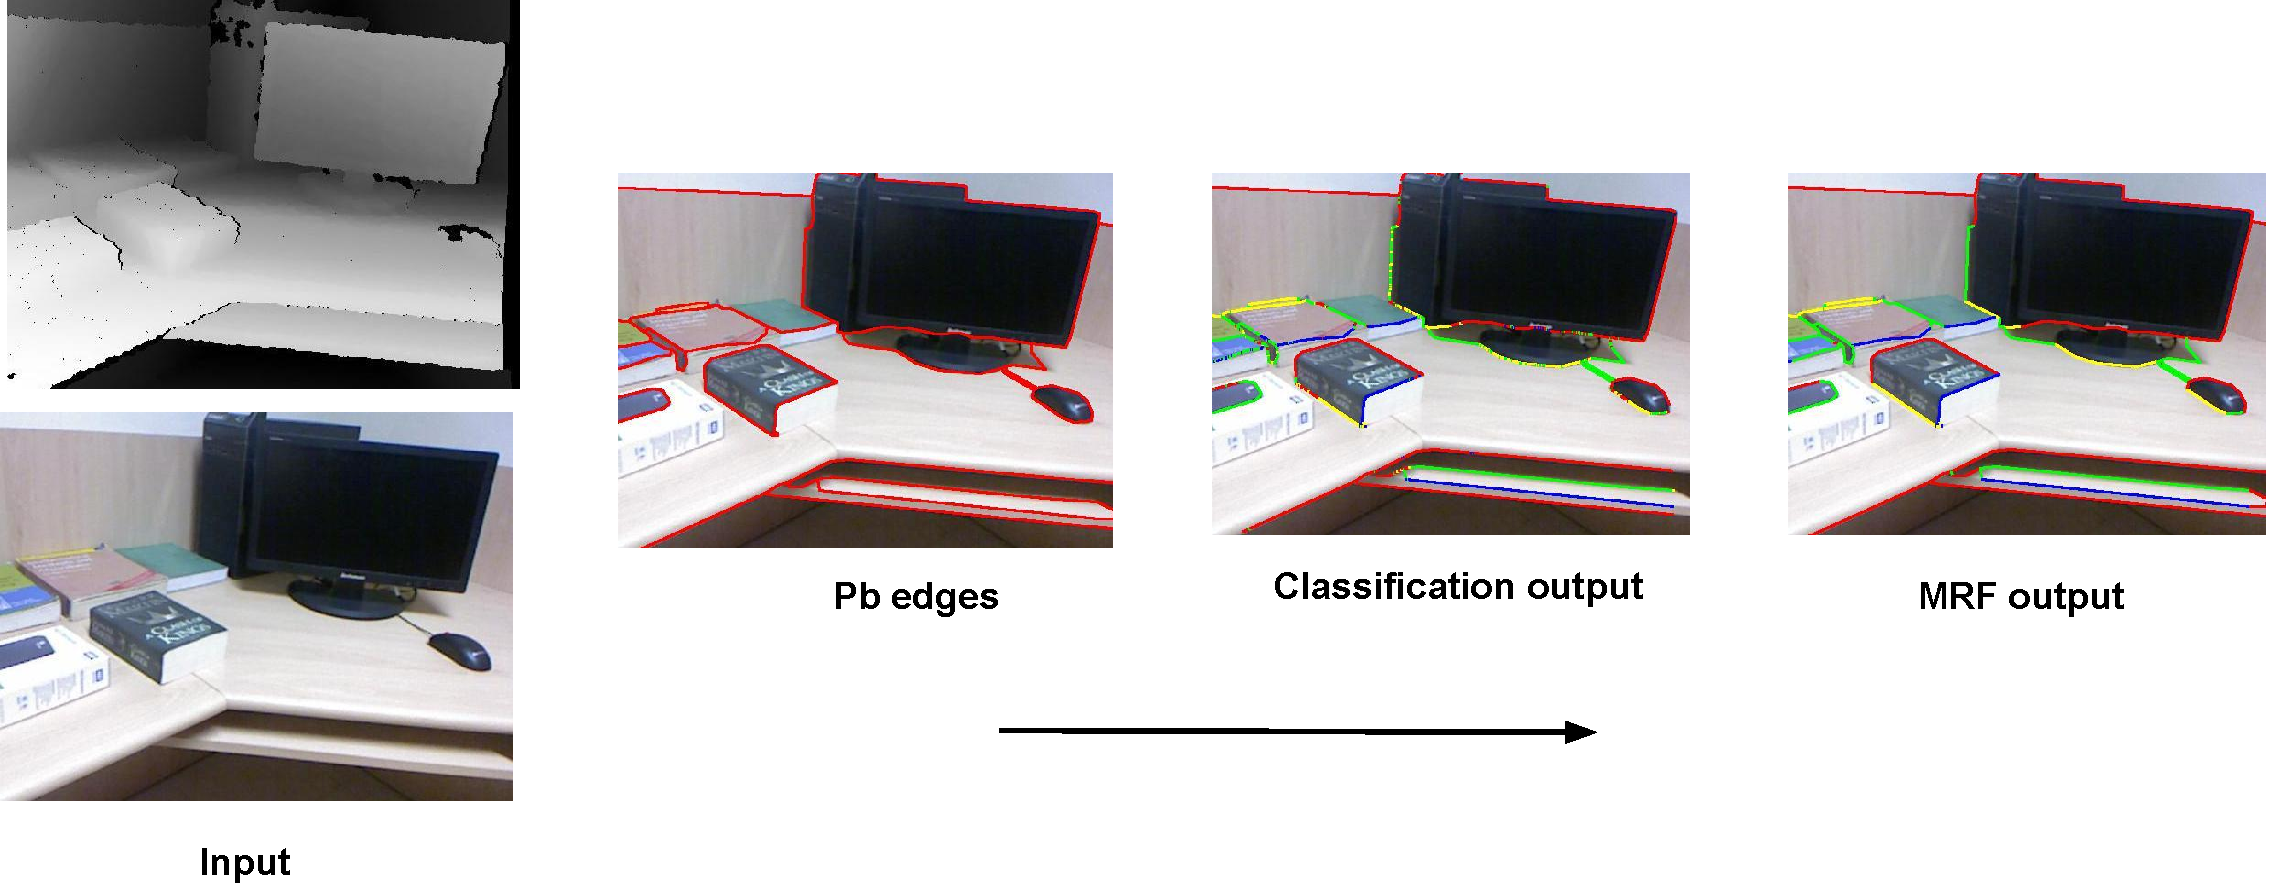
\includegraphics[width=1.0\linewidth]{pipeline_abstract.pdf}
\caption{\it This figure summarizes the pipeline of our approach. It shows RGB and depth maps 
as input (1st image set), with Pb edge detection~\cite{martin2004} (2nd image). The classification and MRF 
outputs are shown in the last two images respectively. Color code: red (occ), green (pln), 
blue (cvx), yellow (ccv).}
\vspace{-2mm}
\label{fig:pipeline}
\end{figure}

\subsection{Contour graph}

Each contour segment is considered as a single entity for 
labeling and is represented as a node in a graph. The junctions between the contour 
segments provide the connectivity information for the graph. Labeling of an object 
boundary is then reduced to labeling of all the nodes in the graph that correspond to 
that specific boundary. Figure~\ref{fig:graph_construction} shows an example, where 
the edge map from a portion of an image is converted into the corresponding contour
graph representation.

We formulate the edge labeling problem as an inference in a graph where the nodes take 
different labels or states. The optimum labeling is achieved by minimizing an energy 
function. Each node can take one of the four labels given by occluding, planar, convex, 
and concave.

Let us consider a graph ${\cal G}=\{{\cal V},{\cal E}\}$, where the vertices of the graph 
correspond to the set of $n$ contour segments; i.e., $c_i \in {\cal V},i=\{1,...,n\}$. The 
edges in the graph are pairs of contour segments. For every junction $J_k$ that falls on 
two contour segments $c_i$ and $c_j$, we have an edge $(c_i,c_j) \in {\cal E}$. Each 
vertex $c_i$ can take four possible states given by ${\cal L}=\{$occ$,$pln$,$cvx$,$ccv$\}$.

\begin{figure}[t]
       \centering
       \subfigure[Edge Links]{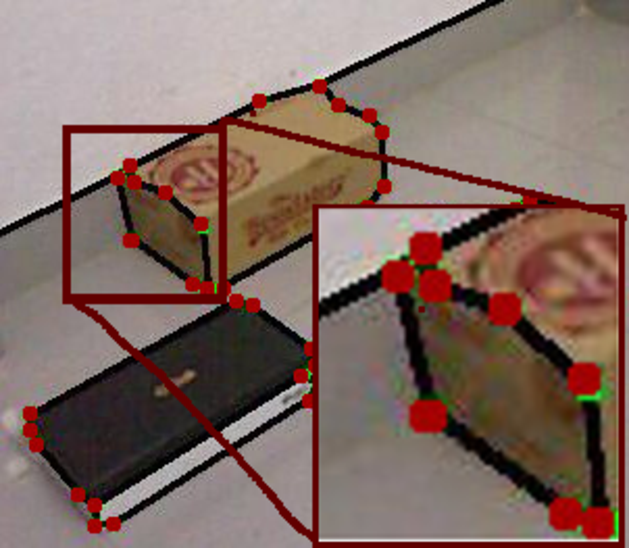
\includegraphics[width=0.27\columnwidth]{images/EdgeLinks.pdf}} \hfill
       \subfigure[Junction Graph]{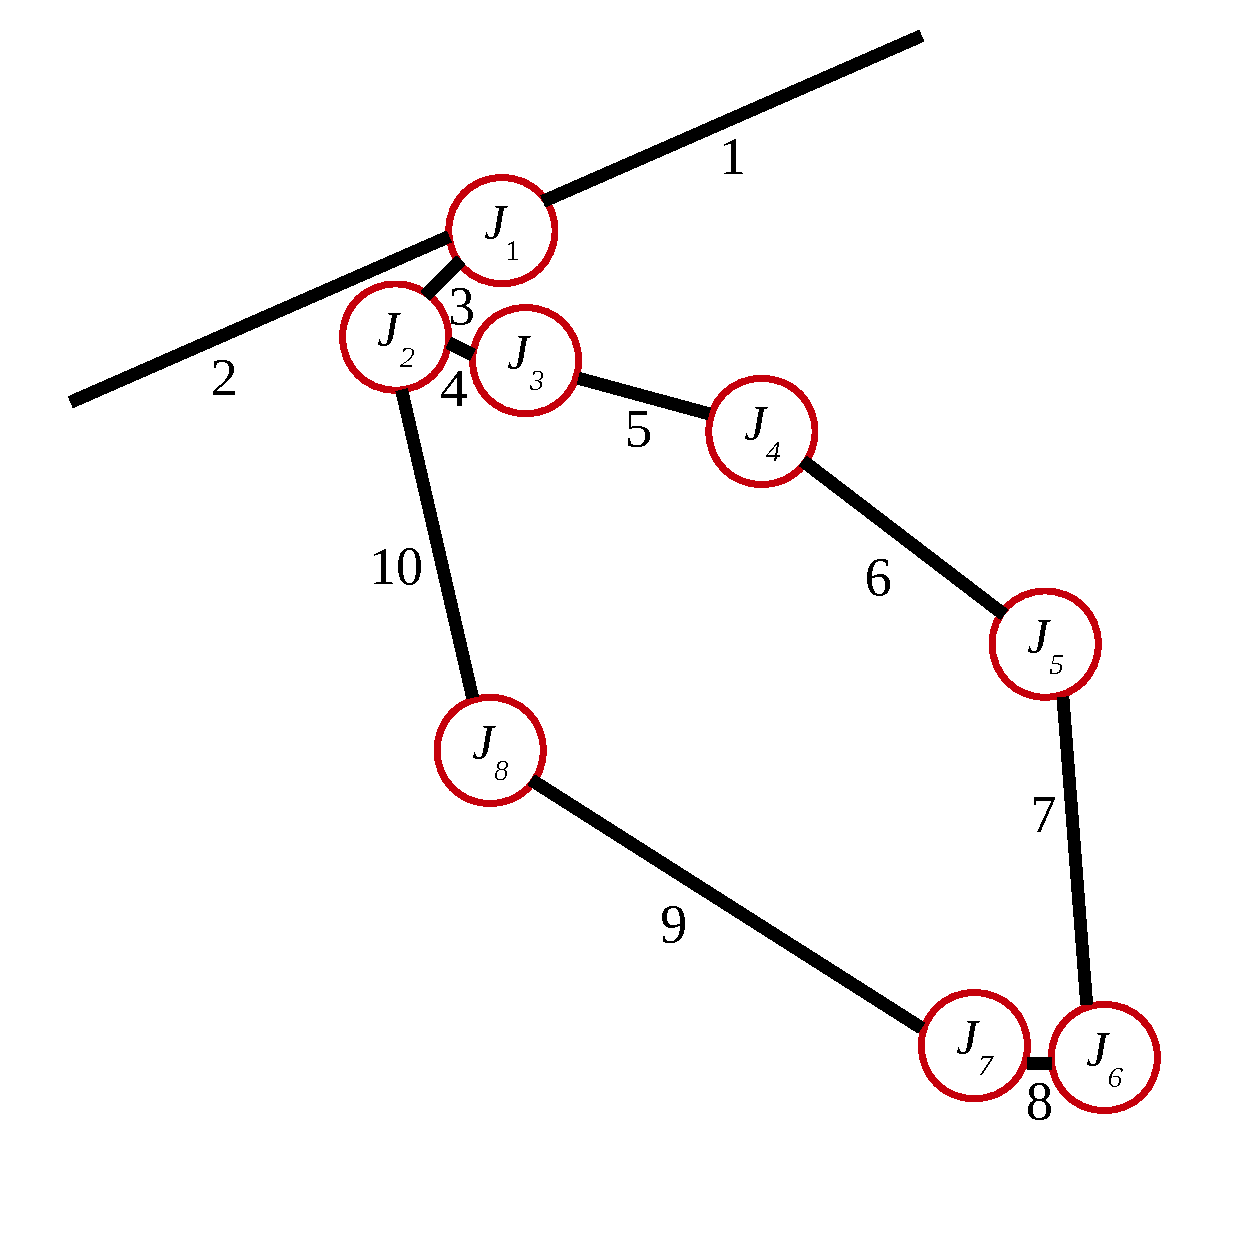
\includegraphics[width=0.27\columnwidth]{images/junctionGraph.pdf}} \hfill
       \subfigure[Contour Graph]{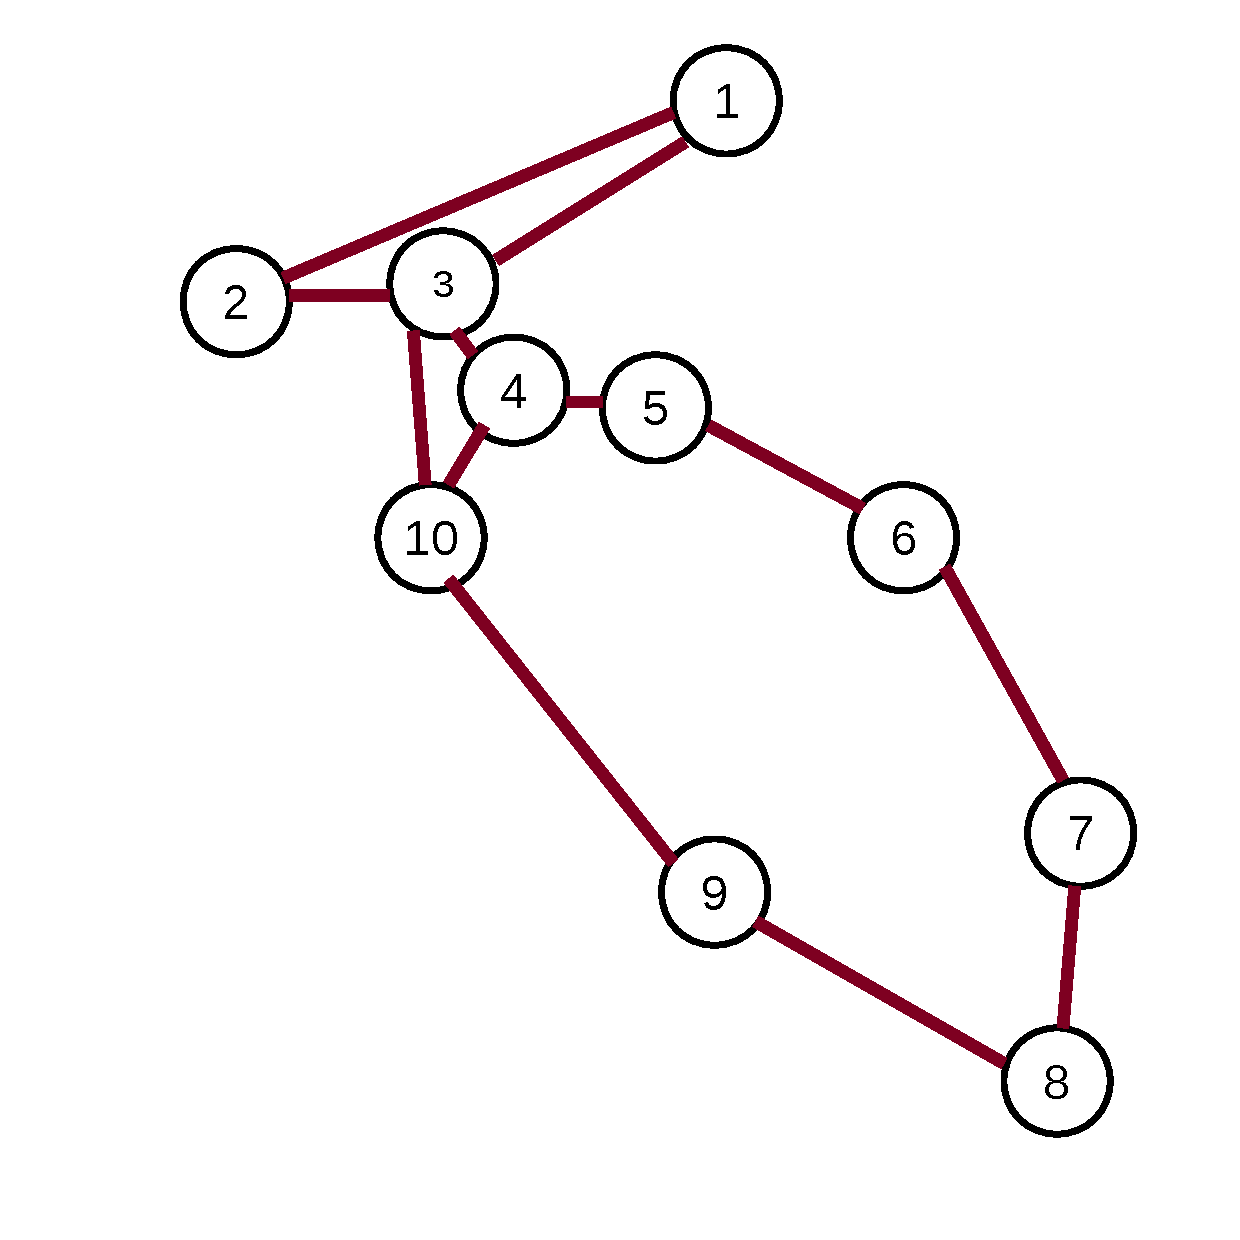
\includegraphics[width=0.27\columnwidth]{images/contourGraph.pdf}} \\
       \caption{\it Contour segments are part of edge links that is bounded by two junctions as shown 
			in (a). In (b), we show a graph where edge junctions are nodes and edge links are edges. In 
			(c), we show a graph with contour segments $c_i$ as nodes and junctions lead to edges between nodes.}
\label{fig:graph_construction}
\end{figure}

To formulate the problem as a labeling problem on an MRF, we need to define unary potentials for
each node $c_i$, as well as the pairwise potentials for every edge in the graph ${\cal G}$.

\subsection{Unary Potentials}

To define the unary potentials of an edge contour $c_i$, we consider the corresponding set of
edge pixels in $c_i$. We define a feature vector for each edge pixel and use a classifier to 
predict its class label. The unary potential of edge contour $c_i$ for label $l$ is 
defined as:
\begin{equation}
\label{unary}
U_l(c_i) = 1 - \frac{N_l}{N_c}
\end{equation}
Here, $N_l$ is the total number of edge pixels on the contour $c_i$ belonging to label $l$. $N_c$ is 
the total number of edge pixels on contour $c_i$. The computation of the feature vector and the 
classification process is described in the following section.

\begin{SCfigure}
       \centering
       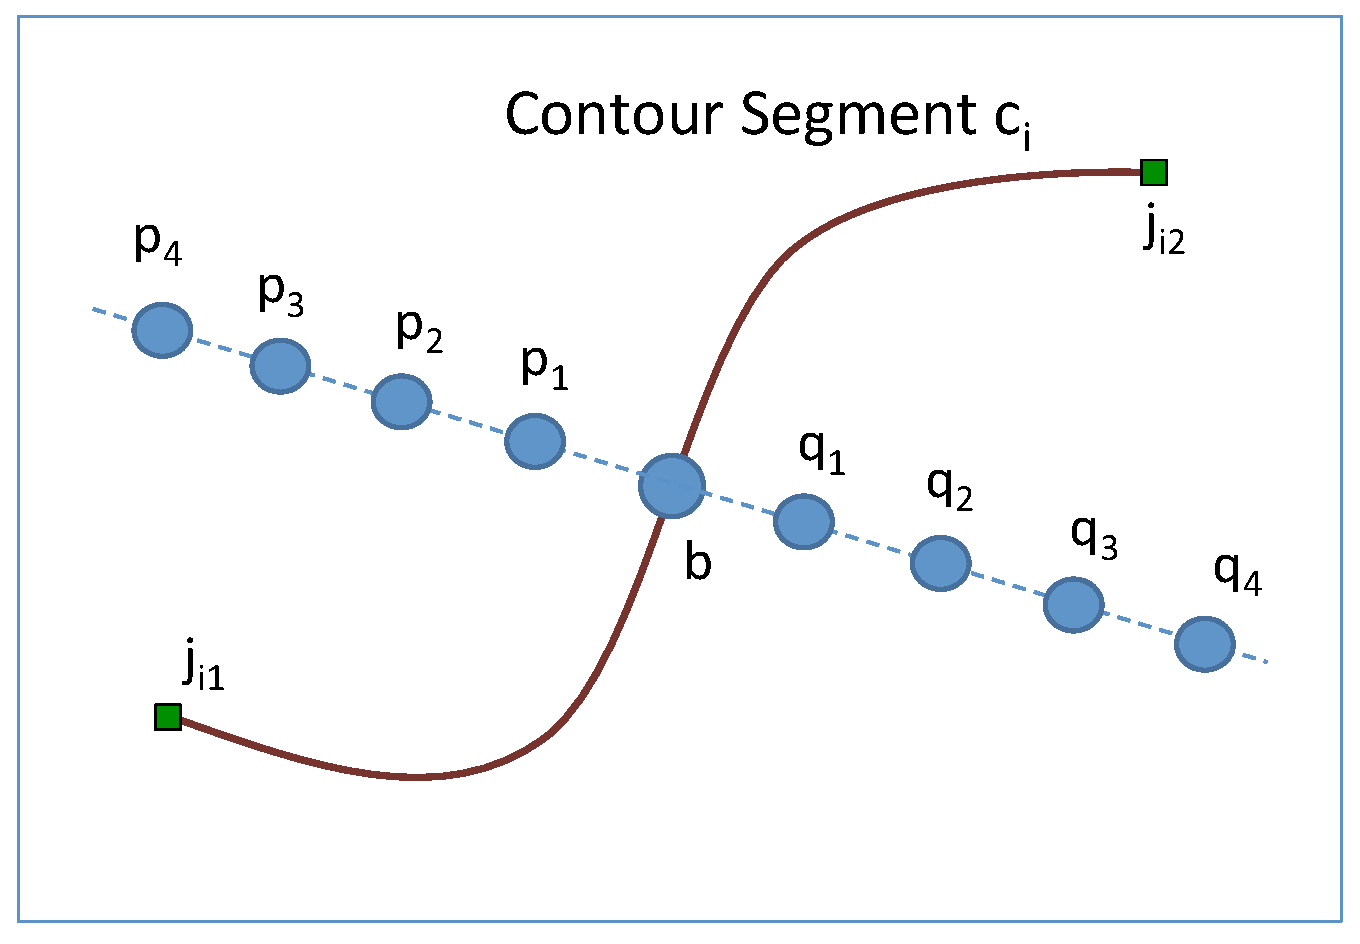
\includegraphics[width=0.40\columnwidth]{images/edgePixels.pdf}
       \caption{\it Edge Pixel Neighborhood: The graph potentials of an edge pixel $b$ are defined based
       on a neighborhood consisting of four pixel on either side of the edge ($p_i$'s and $q_i$'s) on a 
			line perpendicular to the gradient edge direction at $b$.}
\label{fig:edgeNeighbors}
\end{SCfigure}

{\bf The Pixel Classifier:}
Given a contour segment $c_i$, we define its neighborhood properties based on a set of
pixels on either side of the edge as shown in Figure~\ref{fig:edgeNeighbors}. We denote a 
pixel on the contour segment in the image as $b$. We consider $4$ points on either side of 
the edge pixel. These points lie on a line perpendicular to the gradient edge direction at $b$. 
Let the four points on one side be denoted by $(p_1,p_2,p_3,p_4)$ and the other side be 
$(q_1,q_2,q_3,q_4)$. Let $I(p_i)$ denote the RGB color vector at pixel $p_i$.
The corresponding 3D points in the world are denoted using upper 
case letters, $P_i$, $Q_i$ and $B$. The 3D points are obtained using RGBD data. Let $O$ be the 
center of the camera. For a vector $V$, let $<V> = \frac{V}{|V|}$ denote the corresponding 
normalized vector. Let $A.B$ denote the dot product of vectors $A$ and $B$. 
Let ${\cal L}(Q_i,P_j,P_k)$ denote the distance of a point $Q_i$ to the 
3D line joining points $P_j$ and $P_k$. We denote the number of pixels in the neighborhood of 
$b$ with unknown depth values as ${\cal U}(b)$.
	
We briefly describe the role of different elements of the feature vector from the Table~\ref{table:featureVector}.

\begin{table}[h]
\begin{center}
\caption{\it Elements of the feature vector used in pixel-wise edge classifier. Here, the indices 
$i$, $j$ and $k$ vary from 1 to 4.}
\label{table:featureVector}
       \begin{tabular}{|c||c|}
       \hline
        Set Index & Description \\ 
        \hline 
        \hline
				
				1 &
				$<P_i-P_j>.<Q_i-Q_j>$ 
				\\ \hline
				
				2 &
				$\frac{|P_i-Q_i|}{min(|P_i-B|, |Q_i-B|)}$
				\\ \hline
				
				3 &
				$|I(p_i)-I(q_i)|$
				\\ \hline
				
				4 &
				 $<(P_4-B) + (Q_4-B)>.<B-O>$
				\\ \hline
				
				5 & 
				$\frac{|P_i-O|}{|P_{i-1}-O|}$
				\\ \hline
				
				6 &
				${\cal L}(Q_i,P_j,P_k)$
				\\ \hline
				
				7 &
				${\cal U}(b)$
				\\ \hline
				
				8 & 
				$|A-B|,A,B \in \{P_1,..,P_4,B,Q_1,..,Q_4\}$
				\\ \hline
				
				9 & 
				$<P_i-B>.<Q_i-B>$
				\\ \hline
	\end{tabular}
\end{center}
\end{table}


\begin{enumerate}

\item The first set of features denote the dot products based on two vectors on either side of an 
edge pixel. This captures the surface planarity in the neighborhood of an edge pixel. There are six distinct features of this category and are computed from the edge pixel neighborhood (see Figure~\ref{fig:edgeNeighbors}). 
This set of features have high values for planar edge pixels.

\item The second set of features try to capture the depth difference on either side of the edge, 
which helps in finding occlusion edges. The value is expected to be high for occluding edges.

\item The third set captures the normalized color difference between pixels on either side. This 
value is likely to be high for occluding edges.

\item The dot products in the fourth set differentiates between convex and concave labels. 

\item The ratios of distances in the fifth set captures the slopes of surfaces on 
either side from the view point of the camera. This helps in separating convex and concave edges. 
This value would be greater than one for concave and less than one for convex.

\item The sixth set captures the distances from a point to a line. These values are close to zero for planar, 
and nonzero for concave, convex and occluding. For occluding these values are very large.

\item The number of pixels in the neighborhood of an edge with unknown depth values. This number 
is high for occluding edge pixels.

\item The eighth set contains the depth differences between all pairs of points in the set. 

\item The ninth set contains dot products between the pair of vectors originating from $B$ and ending at 
$P_i$ and $Q_i$ respectively.

\end{enumerate}

Given the feature representations of all edge pixels in an image, we train a random forest classifier
with 30 trees that outputs the likelihood for each label. Based on the likelihoods, we identify the class 
label for each pixel.  

\subsection{Inference using graph cuts}

Given the unary and pairwise potentials of each contour segment (node), we will pose the problem
of finding the most likely labels as that of minimizing the total energy over an MRF. A labeling
of the graph, $L$ is defined as an assignment of labels $l_p$ to each node $c_p \in {\cal V}$ in 
the graph ${\cal G}=\{{\cal V},{\cal E}\}$. The data term ${\cal D}(L)$ is a sum
of the unary potentials over all the nodes with respect to the labeling $L$ as shown below:
\begin{equation}
   {\cal D}(L) = \sum_{p=1}^{n} U_{l_p}(c_p)
\end{equation}
The smoothness term ${\cal S}(L)$ is the sum of pairwise potentials over all the neighbors 
$(c_p,c_q) \in {\cal E}$ in the graph ${\cal G}=\{{\cal V},{\cal E}\}$. We use Potts model to define 
the pairwise potential $P_{l_p,l_q}$, which takes a value of 0 for same labels ($l_p=l_q$) and 1 for 
dissimilar ones ($l_p \ne l_q$). The weight factor $W_{l_p,l_q}$ is defined as the cost of assigning 
labels $l_p$ and $l_q$ to any two neighboring nodes $c_p$ and $c_q$. The smoothness terms is shown below:
\begin{equation}
   {\cal S}(L) = \sum_{p,q=1, p \neq q}^{n} W_{l_p,l_q} P_{c_p,c_q}
   \label{eq:datasmooth}
\end{equation}
The total energy $E(L)$ is defined in equation~\ref{eq:E}. The energy function is given by the sum of unary 
and pairwise terms:
\begin{equation}
   \label{eq:E}
   E(L) = \lambda_1  {\cal D}(L) + \lambda_2  {\cal S}(L)
\end{equation}
	
Here, $n$ is the total number of contour segments (nodes) in the graph. The parameters $\lambda_1$ 
and $\lambda_2$ are positive values that control the relative importance of the two terms. For all 
experiments, we use $\lambda_1=1000.0$ and $\lambda_2=12.5$ respectively. The multi-label MRF 
problem is solved using alpha-beta swap~\cite{boykov2001fast}.
% \noindent
% {\bf Algorithm:}
% We use both image and depth cues to infer the labels of edge pixels. We start with a set of 
% edge pixels obtained from an edge detection algorithm and the goal is to assign one of the 
% four labels to each of these edge pixels. Each edge pixel is uniquely mapped to one of the 
% contour segments. Contour segments are sets of linked edge pixels. We formulate the problem 
% as an optimization on a graph constructed using contour segments. We obtain unary features 
% using pixel classifier based on Random forest. We design a feature vector with simple 
% geometric depth comparison features. We use a simple Potts model for pairwise potentials. 
% The individual steps in the algorithm is shown in Figure~\ref{fig:pipeline}.
% \begin{figure}[t]
% \centering
% 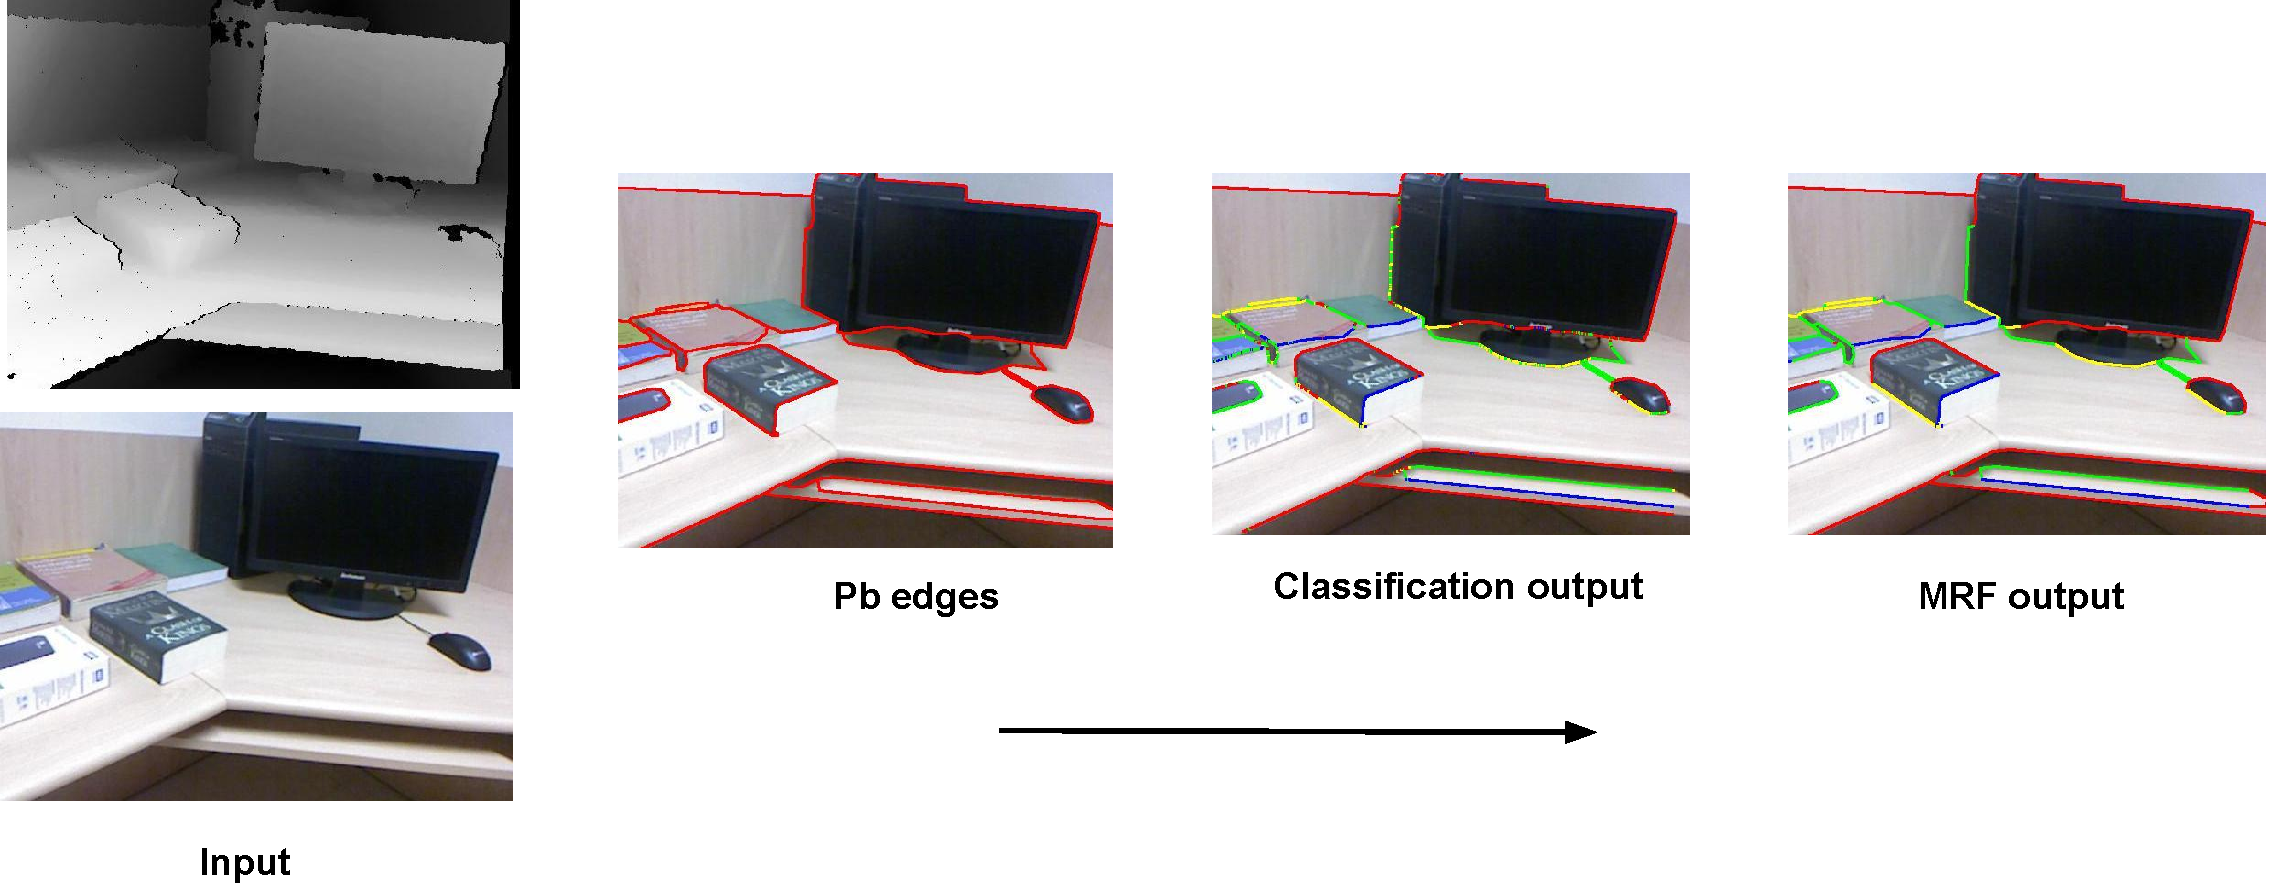
\includegraphics[width=1.0\linewidth]{pipeline_abstract.pdf}
% \caption{\it This figure summarizes the pipeline of our approach. It shows RGB and depth maps 
% as input (1st image set), with Pb edge detection~\cite{martin2004} (2nd image). The classification and MRF 
% outputs are shown in the last two images respectively. Color code: red (occ), green (pln), 
% blue (cvx), yellow (ccv).}
% \vspace{-2mm}
% \label{fig:pipeline}
% \end{figure}


[Contour graph, unary potential (classifier), graph cut..]
\section{Experiments}
[Dataset and annotation, evaluation and numerical results]

{\bf Dataset and Annotation:} We have experimented with multiple edge detectors including Canny~\cite{canny}, Pb~\cite{martin2004} 
and Crisp boundary~\cite{isola14crisp} edge detectors, and finally settled down on the Pb edge detector for our purposes. As noted 
before, the choice of edge detector does not significantly affect the computation of unary potentials and the label assignment. 
However, the connected contour nature of Pb edges makes it easier to define the graph connectivity for MRF formulation. Edge 
detection is followed by edge linking to obtain a set of possible edge contour segments in the image. While this approach provides 
good results, it can be readily replaced by any edge detection algorithm that performs well for the given class of 
images~\cite{edgeDetectSurvey-Koschan}.

\begin{figure}[ht]
   \centering
   \subfigure[RGB]{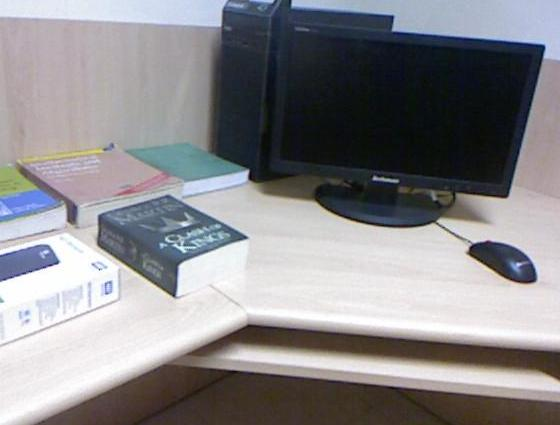
\includegraphics[width=0.25\columnwidth]{results/274.jpg}} \hfill
   \subfigure[Depth Map]{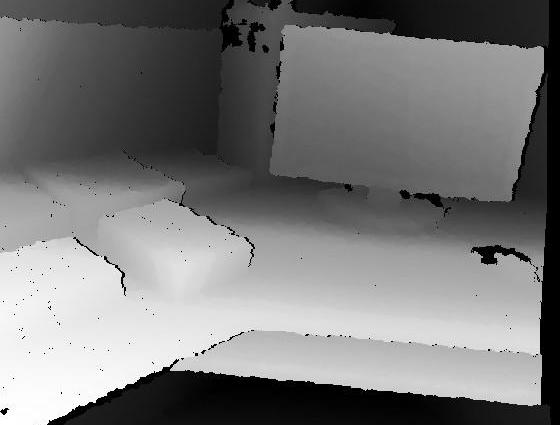
\includegraphics[width=0.25\columnwidth]{results/274_depth.jpg}} \hfill
   \subfigure[Ground truth]{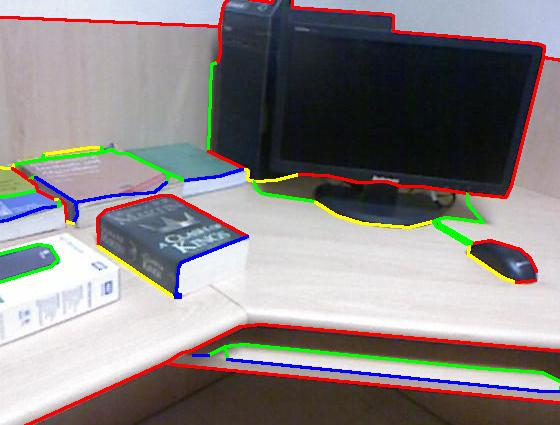
\includegraphics[width=0.25\columnwidth]{results/274_gt.jpg}} \hfill
   \caption{\it Sample image from our dataset showing the RGB image, depth map
   and edge groundtruth. Colors: red (occ), green (pln), blue (cvx), yellow (ccv).}
\label{fig:dataset_depth_GT}
\end{figure}

For quantitative evaluation of the method, we have created an annotated dataset of $500$ RGBD images
of varying complexity. Train to test ratio is 3:2. Though in principle we could use a variety of methods 
to create 3D cues, we use Kinect based images and depth maps in this work. Kinect does not work beyond a 
distance of around four meters. Therefore, our dataset consists of indoor scenes where the objects lie within 
this distance. Our dataset consists of objects such as tables, chairs, cupboard shelves, boxes and household 
objects in addition to walls and floors. We also annotate 100 images from NYU~\cite{Silberman:ECCV12} dataset, 
which include varying scenes from bed-room, living-room, kitchen, bathroom and so on with different complexities. 

For each edge contour, we annotate each of its contour segments with one of the four labels: occlusion, 
convex, concave and planar. The average number of occlusion, planar, convex and concave edges pixels in 
an image in the annotated dataset are $953, 1324, 304$ and $468$ respectively. The corresponding numbers 
for NYU dataset are $1645, 445, 325$ and $399$ respectively. Figure~\ref{fig:dataset_depth_GT} shows an 
annotated example from our dataset. 

\subsection{Evaluation and Numerical Results}

We use recall, precision and F-measure in order to evaluate the performance of the labeling algorithms. 
The average precision, recall and F-measure for each of the edge labels over all the images in the dataset 
is given in Table~\ref{table:evaluation} in addition to results on the NYU dataset. Results for different 
images using the algorithm are given in Figure~\ref{fig:comp2} and Figure~\ref{fig:comp}.

\begin{table}[h]
\begin{center}
\caption{\it Precision, Recall and F-measure for each edge type on our and NYU datasets. $1^{st}$ and $2^{nd}$ 
rows of each set gives the results of our approach and comparison with ~\cite{gupta13Perceptual}. The $3^{rd}$ 
row in each set shows the results of our approach on NYU dataset.}
\label{table:evaluation}
       \begin{tabular}{|c||c|c|c|c|}
       \hline
        & Occluding & Planar & Convex & Concave \\ 
        \hline 
        \hline
	Recall & {\bf 0.85} & {\bf 0.92} & {\bf 0.70} & {\bf 0.78} \\ \hline 
	Gupta {\em et al.}~\cite{gupta13Perceptual} Recall & 0.70 & 0.84 & 0.52 & 0.67 \\ \hline 
	Our Recall on NYU & $0.76$ & $0.85$ & $0.56$ & $0.69$ \\ \hline  \hline
	Precision &  {\bf 0.86 } & {\bf 0.81} & {\bf 0.93} &{\bf 0.89} \\ \hline 
	Gupta {\em et al.}~\cite{gupta13Perceptual} Precision & 0.71 & 0.75 & 0.72 & 0.71 \\ \hline
	Our Precision on NYU & $0.79$ & $0.80$ & $0.77$ & $0.71$ \\ \hline   \hline
	F-measure & {\bf 0.86 } &  {\bf 0.86 } &  {\bf 0.80 } &  {\bf 0.83 } \\ \hline 
	Gupta {\em et al.}~\cite{gupta13Perceptual} F-measure & 0.71 & 0.79 & 0.61 & 0.69 \\ \hline 
	Our F-measure on NYU & $0.77$ & $0.83$ & $0.65$ & $0.70$ \\ \hline 
\end{tabular}
\end{center}
\end{table}
\vspace{-5mm}

\begin{table}[h]
\parbox{.4\linewidth}{
\centering
\caption{\it Confusion matrix across the four classes.  The numbers given
are the average number of edge pixels per image.}
\label{table:confusion}
       \begin{tabular}{|c||c|c|c|c|}
       \hline
        & Occ & Pln & Cvx & Ccv \\ 
        \hline 
        \hline
	Occ & 677 & 100 & 5 & 11 \\ \hline 
	Pln & 53 & 993 & 10 & 27 \\ \hline 
	Cvx & 27 & 58 & 201 & 2 \\ \hline 
	Ccv & 28 & 70 & 1 & 344 \\ \hline 
\end{tabular}
}
\hfill
\parbox{.55\linewidth}{
\centering
\caption{\it Precision, recall and F-measure for each edge type without and with
pairwise potentials.}
\label{table:compare}
       \begin{tabular}{|c||c|c|c|c|}
       \hline
        & Occ & Pln & Cvx & Ccv \\ 
        \hline 
        \hline
	Pixel Recall & 0.82 & 0.87 & 0.69 & 0.75 \\ \hline 
%	Contour Recall & -.-- & -.-- & -.-- & -.-- \\ \hline 
	Final Recall & {\bf 0.85} & {\bf 0.92} & {\bf 0.70} & {\bf 0.78} \\ \hline \hline
	Pixel Precision & 0.84 & {\bf 0.85} & 0.90 &  0.86 \\ \hline 
%	Contour Precision & -.-- & -.-- & -.-- & -.-- \\ \hline 
	Final Precision & {\bf 0.86} &  0.81 & {\bf 0.93} & {\bf 0.89} \\ \hline \hline
	Pixel F-measure & 0.83 & 0.86 & 0.78 & 0.80 \\ \hline 
%	Contour F-measure & -.-- & -.-- & -.-- & -.-- \\ \hline 
	Final F-measure & {\bf 0.86} & {\bf 0.86} & {\bf 0.80} & {\bf 0.83} \\ \hline 
\end{tabular}
}
\end{table}

To understand the effect of unary versus pairwise potentials on the precision and recall measures, we
look at the effect of classification of edge pixels and edge contour segments using only the unary potentials,
without the pairwise terms. Table~\ref{table:compare} shows the resulting precision, recall and F-score
values over the whole database. For convenience of comparison, we have also included the results using
the pairwise terms. We get an average F-score of 0.82 on the classification results for our 
data set. The use of smoothness constraints in the MRF achieves an F-score of 0.84.

We compare the proposed approach with the semantic labeling of edges obtained by 
Gupta {\em et al.}~\cite{gupta13Perceptual}, by computing their results on our dataset of annotated 
edges. Note that their work provides three labels (occluding, convex and concave). Since our dataset 
contains planar edges also, we perform a straight-forward extension of their approach to $4$ labels 
for a fair comparison.

For evaluation purposes, we consider only those pixels in the cropped range $41-600\times46-470$ to 
remove the area where depth information is mostly missing in the Kinect depth map. This was done to 
be consistent with \cite{gupta13Perceptual} in the data used for comparison. Figure~\ref{fig:comp2}, 
Figure~\ref{fig:comp} and table~\ref{table:evaluation} provide qualitative and quantitative comparisons 
of the outputs of the two approaches. It can be seen that our approach produces superior results. 
We see that our approach labels the edges correctly even when they occur extremely close to another type of edge. For \textit{e.g.}, in result (d) of figure~\ref{fig:comp}, the rightmost convex edge got correctly 
classified while the approach by Gupta {\em et al.}~\cite{gupta13Perceptual} fails to do so. Similar results 
can be seen in much of the complex images in the NYU dataset (see figure~\ref{fig:nyuResults}). 

We see that the algorithm achieves high precision for each of the edge types. The recalls are also 
high except for convex and concave edges. This is primarily due to the fact that we have several complex 
scenes in our dataset where a convex/concave edge does not have good depth quantization or do not have 
enough depth values registered around it. We are able to correctly classify complex convex/concave edges 
even with narrow regions having steep slope on either sides of the edge, provided the depth map is good. 
The NYU dataset contains complex scenes with glass windows and table heads for which Kinect fails to 
register the depth accurately. While this results in lower recall for convex and concave edges, we 
achieve an average F-score of $0.74$ for the NYU dataset.

On detailed analysis, the primary causes of errors in our approach were found to be: i) missing depth 
values from Kinect and ii) very small depth differences for occluding edges. While the first problem may 
be solved using better sensors and using image based potentials, the second would require a higher level 
understanding of the scene and objects. The proposed algorithm can be extended to work with SFM point 
clouds as well. The depth map in SFM can be easily created using the camera matrices of images and the 
point cloud. The main challenge here is that SFM point cloud is sparser than Kinect. Therefore, the depth 
and normal information may not be as reliable as that of Kinect.

\begin{figure*}[ht]
   \centering

   \subfigure{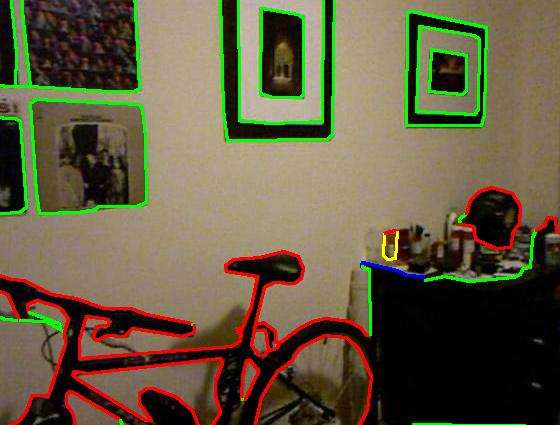
\includegraphics[width=0.19\columnwidth]{results/557_GT.jpg}} \hfill
   \subfigure{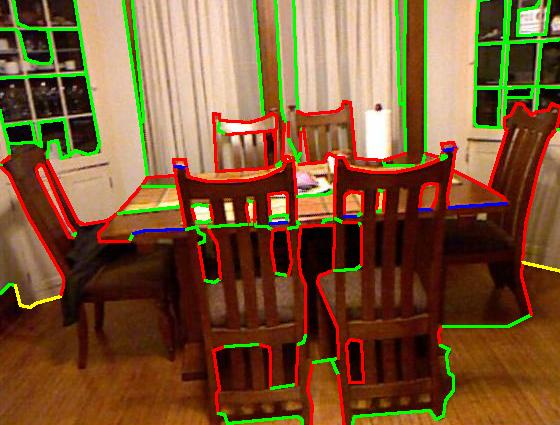
\includegraphics[width=0.19\columnwidth]{results/637_GT.jpg}} \hfill
   \subfigure{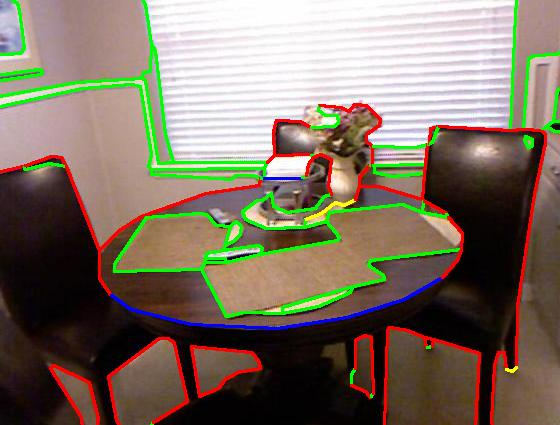
\includegraphics[width=0.19\columnwidth]{results/734_GT.jpg}} \hfill
   \subfigure{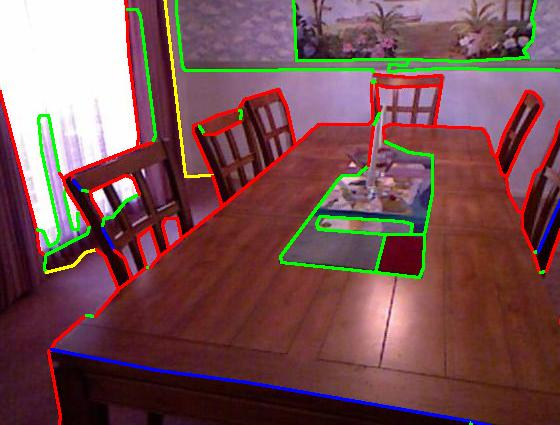
\includegraphics[width=0.19\columnwidth]{results/941_GT.jpg}} \hfill
   \subfigure{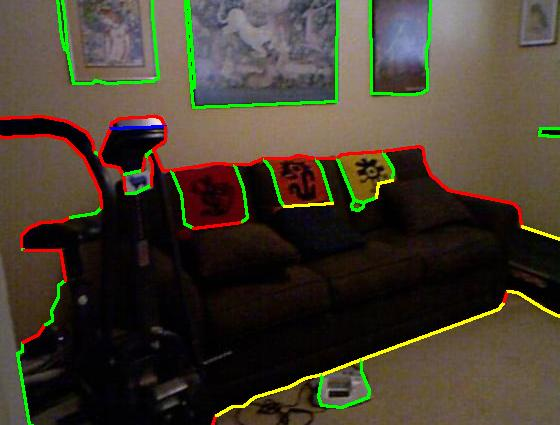
\includegraphics[width=0.19\columnwidth]{results/934_GT.jpg}} \\
   \addtocounter{subfigure}{-5}
   \subfigure{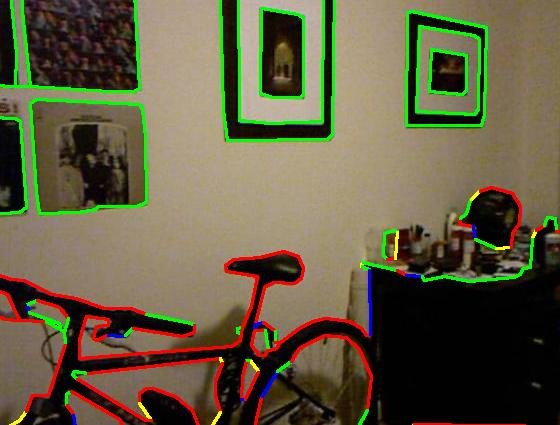
\includegraphics[width=0.19\columnwidth]{results/557_MRF.jpg}} \hfill
   \subfigure{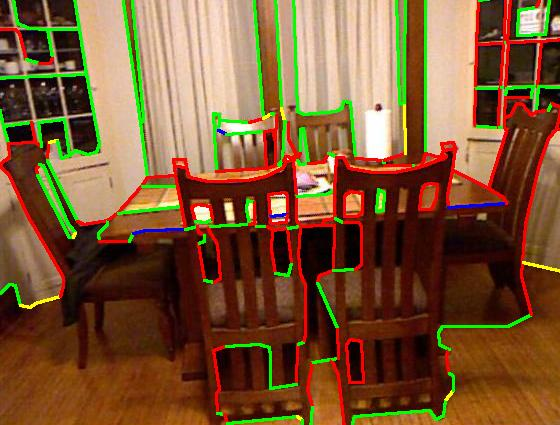
\includegraphics[width=0.19\columnwidth]{results/637_MRF.jpg}} \hfill
   \subfigure{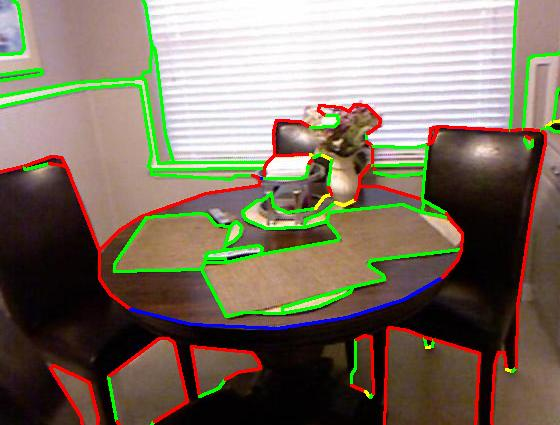
\includegraphics[width=0.19\columnwidth]{results/734_MRF.jpg}} \hfill
   \subfigure{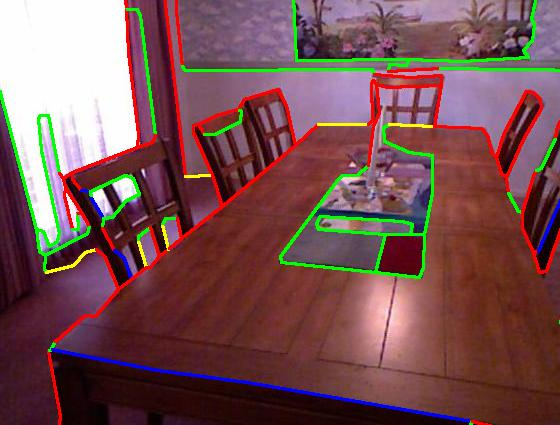
\includegraphics[width=0.19\columnwidth]{results/941_MRF.jpg}} \hfill
   \subfigure{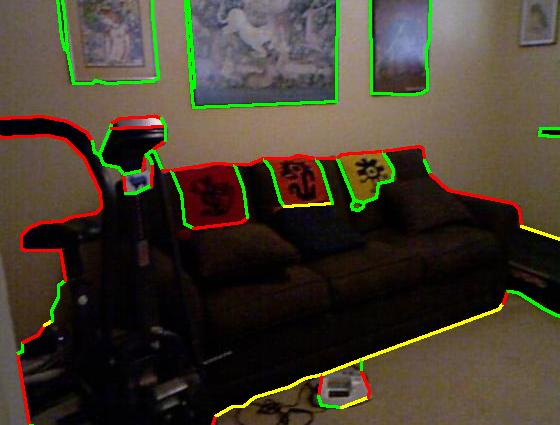
\includegraphics[width=0.19\columnwidth]{results/934_MRF.jpg}} \\
   \addtocounter{subfigure}{-5}

   \caption{\it NYU dataset results : Ground truths (above) and the corresponding results from our approach (below).
   Color code: red (occ), green (pln), blue (cvx), yellow (ccv).}
\label{fig:nyuResults}
\end{figure*}

   \begin{figure*}[ht]
   \centering


   \subfigure{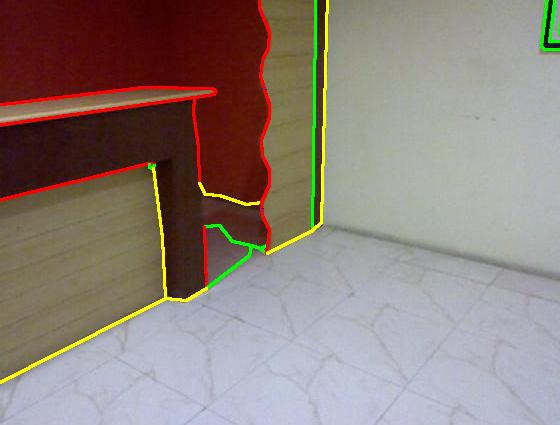
\includegraphics[width=0.16\columnwidth]{results/143_gt.jpg}} \hfill
    \subfigure{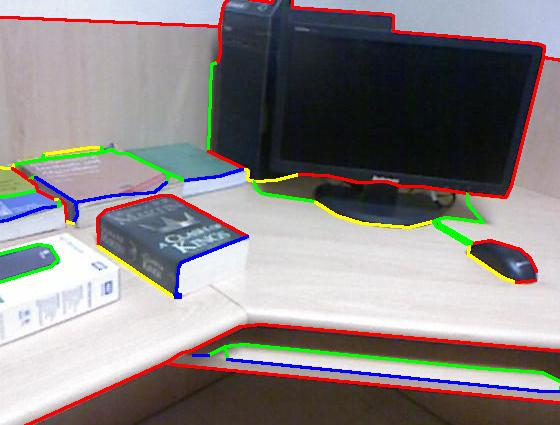
\includegraphics[width=0.16\columnwidth]{results/274_gt.jpg}}  \hfill
   \subfigure{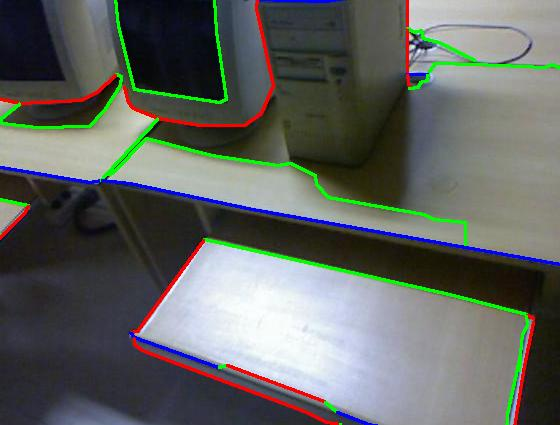
\includegraphics[width=0.16\columnwidth]{supplementary/364_gt.jpg}} \hfill
  \subfigure{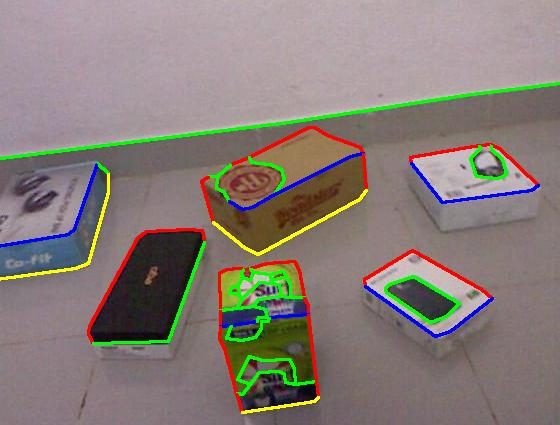
\includegraphics[width=0.17\columnwidth]{results/214_gt.jpg}} \hfill
   \subfigure{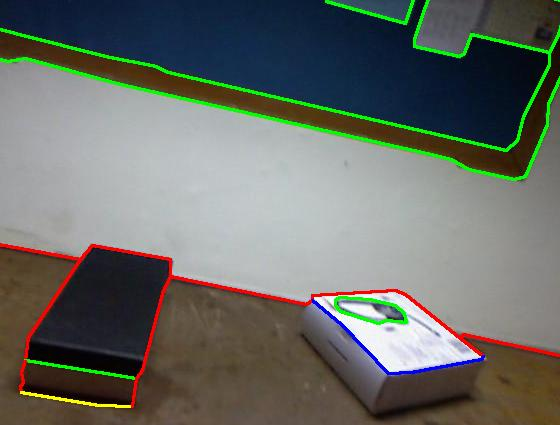
\includegraphics[width=0.17\columnwidth]{supplementary/90_gt.jpg}} \\   
  \subfigure{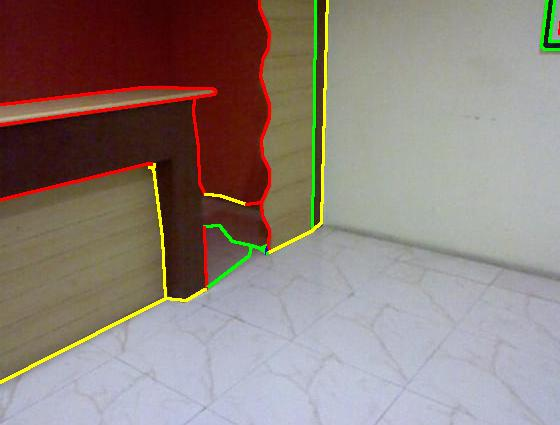
\includegraphics[width=0.16\columnwidth]{results/143_graphcut.jpg}} \hfill
   \subfigure{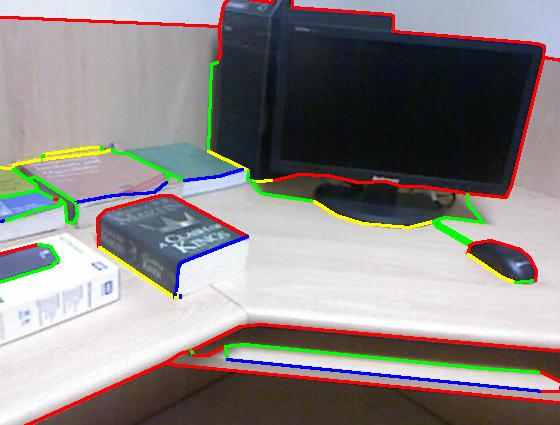
\includegraphics[width=0.16\columnwidth]{results/274_graphcut.jpg}} \hfill
   \subfigure{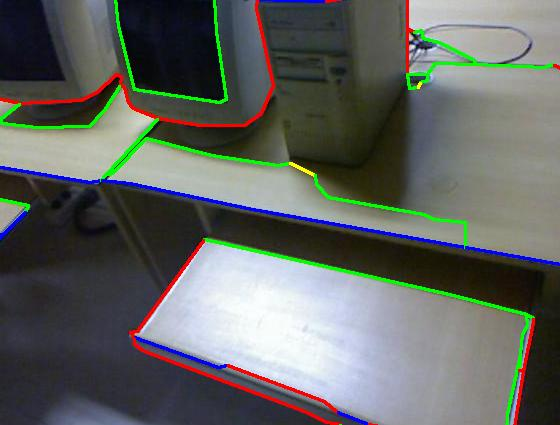
\includegraphics[width=0.16\columnwidth]{supplementary/364_graphcut.jpg}} \hfill
   \subfigure{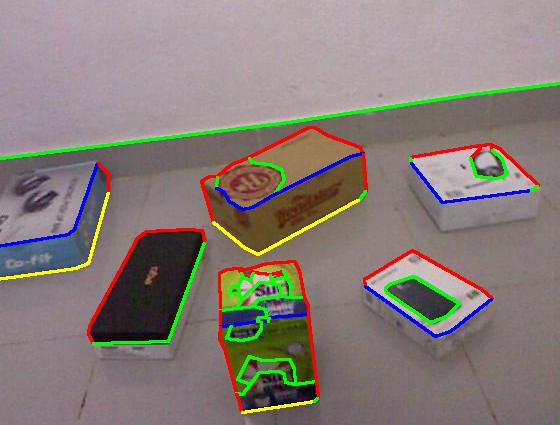
\includegraphics[width=0.17\columnwidth]{results/214_graphcut.jpg}} \hfill
   \subfigure{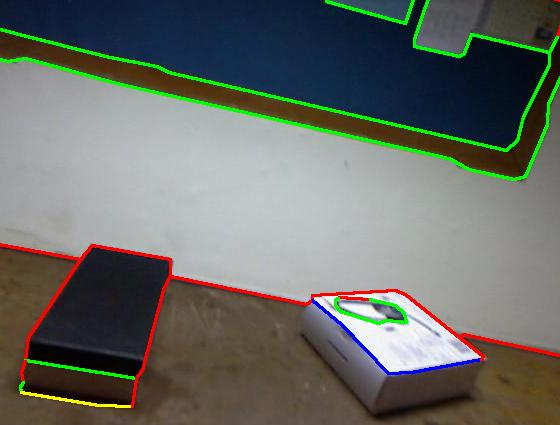
\includegraphics[width=0.17\columnwidth]{supplementary/90_graphcut.jpg}} \\ 
   \addtocounter{subfigure}{-5}
   \subfigure[]{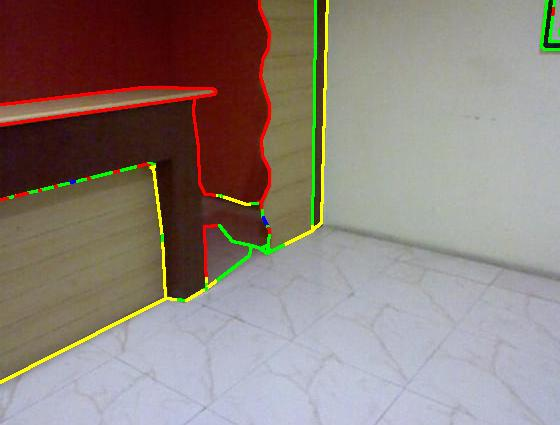
\includegraphics[width=0.16\columnwidth]{results/Gupta/143.jpg}} \hfill
  \subfigure[]{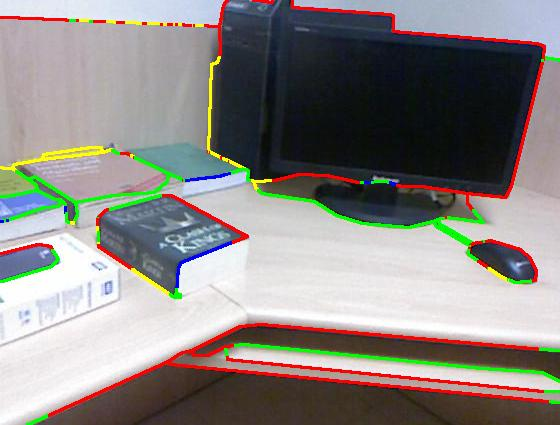
\includegraphics[width=0.16\columnwidth]{results/Gupta/274.jpg}} \hfill
  \subfigure[]{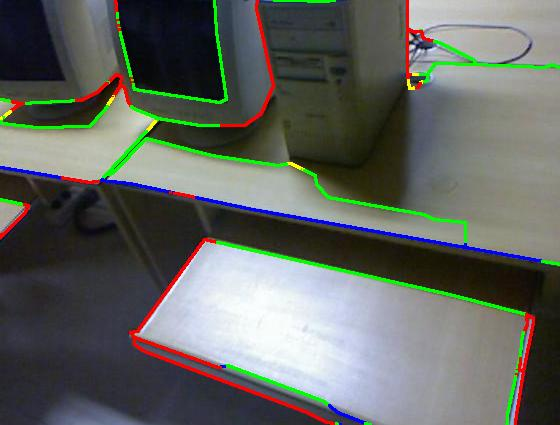
\includegraphics[width=0.16\columnwidth]{results/Gupta/364.jpg}} \hfill
    \subfigure[]{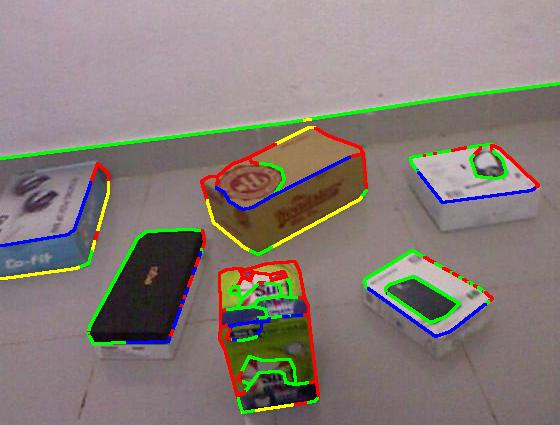
\includegraphics[width=0.17\columnwidth]{results/Gupta/214.jpg}}  \hfill
   \subfigure[]{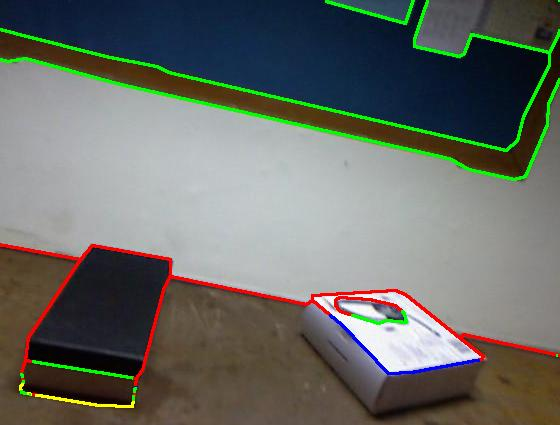
\includegraphics[width=0.17\columnwidth]{results/Gupta/90.jpg}} \\
  \caption{\it Ground truths (above) and the corresponding results from our approach ($2^{nd}$ row)
   and Gupta {\em et al.}~\cite{gupta13Perceptual} ($3^{rd}$ row). Color code: red (occ), green (pln), 
   blue (cvx), yellow (ccv).}
\label{fig:comp2}
\end{figure*}

\begin{figure*}[ht]
   \centering

   \subfigure{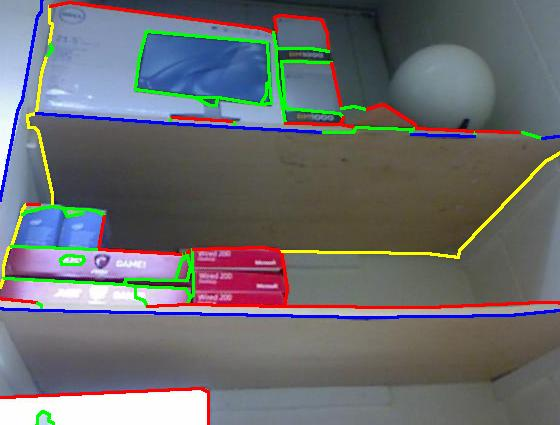
\includegraphics[width=0.19\columnwidth]{results/387_GT.jpg}} \hfill
   \subfigure{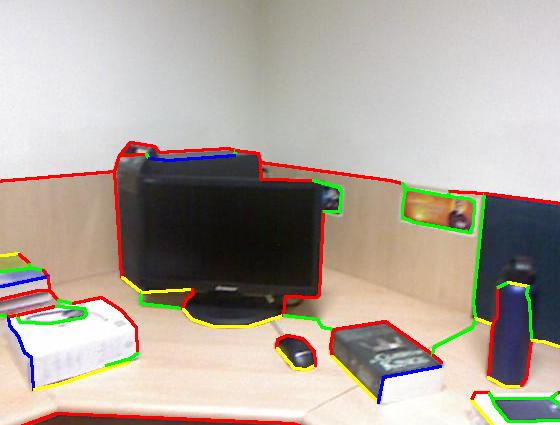
\includegraphics[width=0.19\columnwidth]{results/248_GT.jpg}} \hfill
   %\subfigure{\includegraphics[width=0.19\columnwidth]{results/332_GT.jpg}} \hfill
   \subfigure{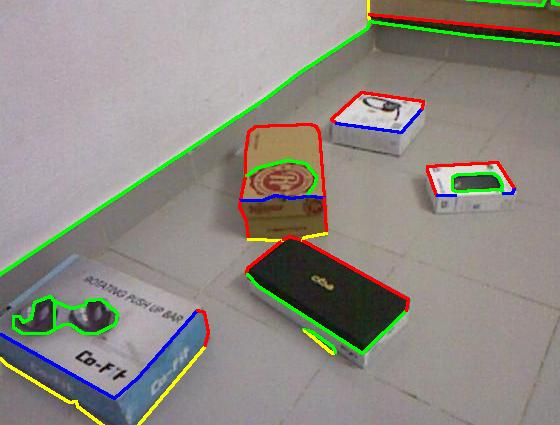
\includegraphics[width=0.19\columnwidth]{results/228_GT.jpg}} \hfill
   \subfigure{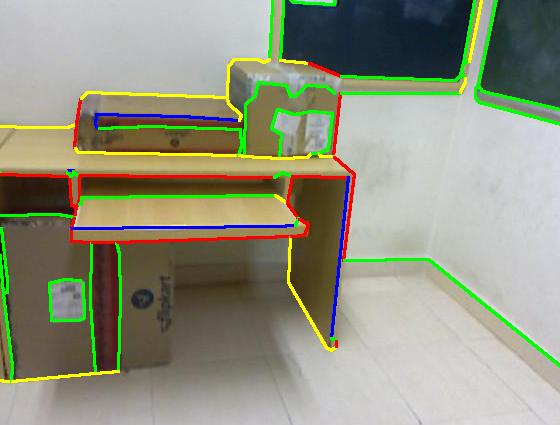
\includegraphics[width=0.19\columnwidth]{results/410_GT.jpg}} \hfill
   %\subfigure{\includegraphics[width=0.19\columnwidth]{results/432_GT.jpg}} \hfill
   \subfigure{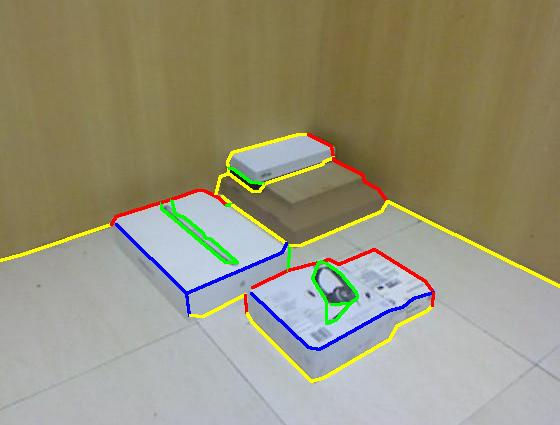
\includegraphics[width=0.19\columnwidth]{results/464_GT.jpg}} \\

   \subfigure{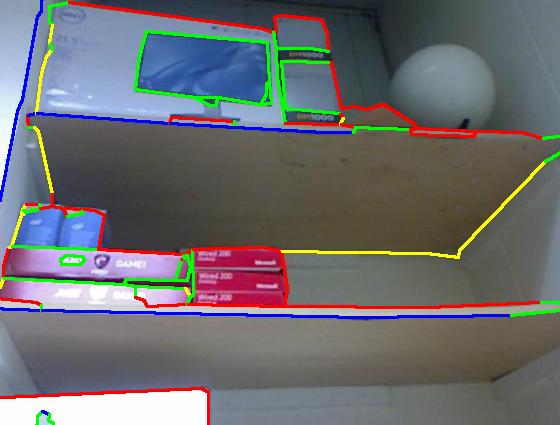
\includegraphics[width=0.19\columnwidth]{results/387_MRF.jpg}} \hfill
   \subfigure{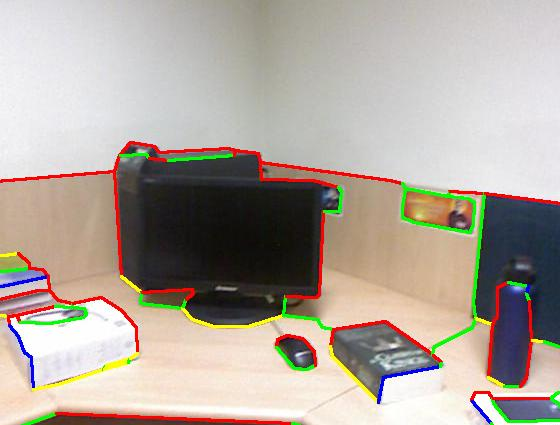
\includegraphics[width=0.19\columnwidth]{results/248_MRF.jpg}} \hfill
   %\subfigure{\includegraphics[width=0.19\columnwidth]{results/332_MRF.jpg}} \hfill
   \subfigure{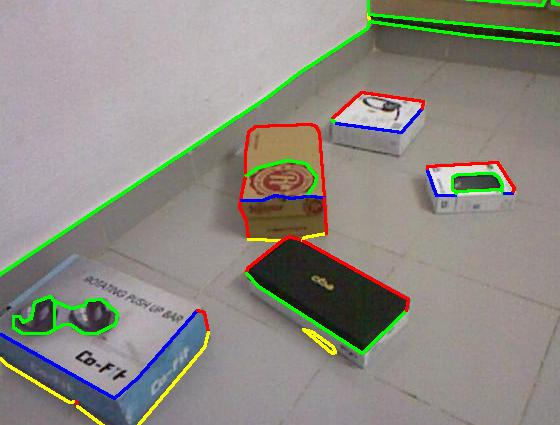
\includegraphics[width=0.19\columnwidth]{results/228_MRF.jpg}} \hfill
   \subfigure{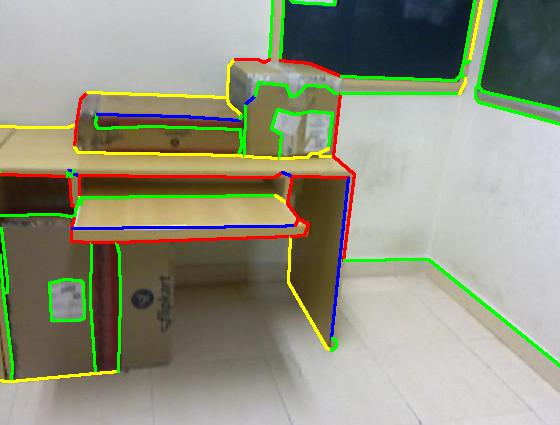
\includegraphics[width=0.19\columnwidth]{results/410_MRF.jpg}} \hfill
   %\subfigure{\includegraphics[width=0.19\columnwidth]{results/432_MRF.jpg}} \hfill
   \subfigure{\includegraphics[width=0.19\columnwidth]{results/464_MRF.jpg}} \\ 
   \addtocounter{subfigure}{-10}
   \subfigure[]{\includegraphics[width=0.19\columnwidth]{results/Gupta/387.jpg}} \hfill
   \subfigure[]{\includegraphics[width=0.19\columnwidth]{results/Gupta/248.jpg}} \hfill
   %\subfigure[]{\includegraphics[width=0.19\columnwidth]{results/Gupta/332.jpg}} \hfill
   \subfigure[]{\includegraphics[width=0.19\columnwidth]{results/Gupta/228.jpg}} \hfill
   \subfigure[]{\includegraphics[width=0.19\columnwidth]{results/Gupta/410.jpg}} \hfill
   %\subfigure[]{\includegraphics[width=0.19\columnwidth]{results/Gupta/432.jpg}} \hfill
   \subfigure[]{\includegraphics[width=0.19\columnwidth]{results/Gupta/464.jpg}} \\ 

   \subfigure{\includegraphics[width=0.17\columnwidth]{supplementary/131_gt.jpg}} \hfill
   \subfigure{\includegraphics[width=0.17\columnwidth]{supplementary/394_gt.jpg}} \hfill
   \subfigure{\includegraphics[width=0.17\columnwidth]{supplementary/407_gt.jpg}} \hfill
  \subfigure{\includegraphics[width=0.17\columnwidth]{supplementary/56_gt.jpg}} \hfill
   \subfigure{\includegraphics[width=0.17\columnwidth]{supplementary/432_gt.jpg}} \\   
   \subfigure{\includegraphics[width=0.17\columnwidth]{supplementary/131_graphcut.jpg}} \hfill
   \subfigure{\includegraphics[width=0.17\columnwidth]{supplementary/394_graphcut.jpg}} \hfill
   \subfigure{\includegraphics[width=0.17\columnwidth]{supplementary/407_graphcut.jpg}} \hfill
   \subfigure{\includegraphics[width=0.17\columnwidth]{supplementary/56_graphcut.jpg}} \hfill
   \subfigure{\includegraphics[width=0.17\columnwidth]{supplementary/432_graphcut.jpg}} \\ 
   \addtocounter{subfigure}{-10}
   \subfigure[]{\includegraphics[width=0.17\columnwidth]{results/Gupta/131.jpg}} \hfill
   \subfigure[]{\includegraphics[width=0.17\columnwidth]{results/Gupta/394.jpg}} \hfill
   \subfigure[]{\includegraphics[width=0.17\columnwidth]{results/Gupta/407.jpg}} \hfill
    \subfigure[]{\includegraphics[width=0.17\columnwidth]{results/Gupta/56.jpg}}  \hfill
   \subfigure[]{\includegraphics[width=0.17\columnwidth]{results/Gupta/432.jpg}} \\
  \caption{\it Ground truths (above) and the corresponding results from our approach ($2^{nd}$ row)
   and Gupta {\em et al.}~\cite{gupta13Perceptual} ($3^{rd}$ row). Color code: red (occ), green (pln), 
   blue (cvx), yellow (ccv).}
\label{fig:comp}
\end{figure*}


